% You should title the file with a .tex extension (hw1.tex, for example)
\documentclass[a4paper, 11pt]{article}

\usepackage{amsmath}
\usepackage{amssymb}
\usepackage{fancyhdr}
\usepackage{graphicx}

\usepackage[margin=1in]{geometry}

\newcommand{\question}[2] {\vspace{.25in} \hrule\vspace{0.5em}
\noindent{\bf #1: #2} \vspace{0.5em}
\hrule \vspace{.10in}}
\renewcommand{\part}[1] {\vspace{.10in} {\bf (#1)}}

\newcommand{\myname}{Natthakan Euaumpon}
\newcommand{\myemail}{natthakaneuaumpon@gmail.com}
\newcommand{\myhwnum}{1}

\setlength{\parindent}{0pt}
\setlength{\parskip}{5pt plus 1pt}
 
\pagestyle{fancyplain}
\lhead{\fancyplain{}{\textbf{HW\myhwnum}}}      % Note the different brackets!
\rhead{\fancyplain{}{\myname\\ \myemail}}
\chead{\fancyplain{}{ICCS240 }}

\begin{document}

\medskip                        % Skip a "medium" amount of space
                                % (latex determines what medium is)
                                % Also try: \bigskip, \littleskip

\thispagestyle{plain}
\begin{center}                  % Center the following lines
{\Large ICCS240: Assignment \myhwnum} \\
\myname \\
\myemail \\
February 2020 \\
\end{center}

\question{1}{Warm-upQuestions}
\part{1}{How many relations over S,T are there?}\\ 
$2^{mn}$\\

\part{2}{How many functions from S to T are there}\\
$m^n$

\question{2}{Relational Algebra}

\part{1}  {$\Pi_{B}(R\bowtie S) = \Pi_{B}(R)\cap \Pi_{B}(S)$}\\
By definition of natural join in set representation,\\
Let K be result set of the natural join between sets R ans S, T[A] be the tuples taken from table A and T[B] denotes the table taken from table B.\\
$K = R\bowtie S$\\
$K =\{T\in B_SB_R|T[S]\in s \wedge T[B_R]\in R\}$
We can project the result set, K\\
$\Pi_B (K) = \{T[Bs]\in S \wedge T[B_R] \in R\}$
We want to show that the intersection given yield the same result as the natural join.\\
$R \cap S = \{T|T\in R and T\in S\}$\\
We can project this as:\\
$\Pi_{B}[R] \cap \Pi_{B}[S] = \{T|T[B] ans T[B] \in S\}$

\question{3}{E/R  Diagram and Relational Model}
\part{1}{E/R Diagram}\\
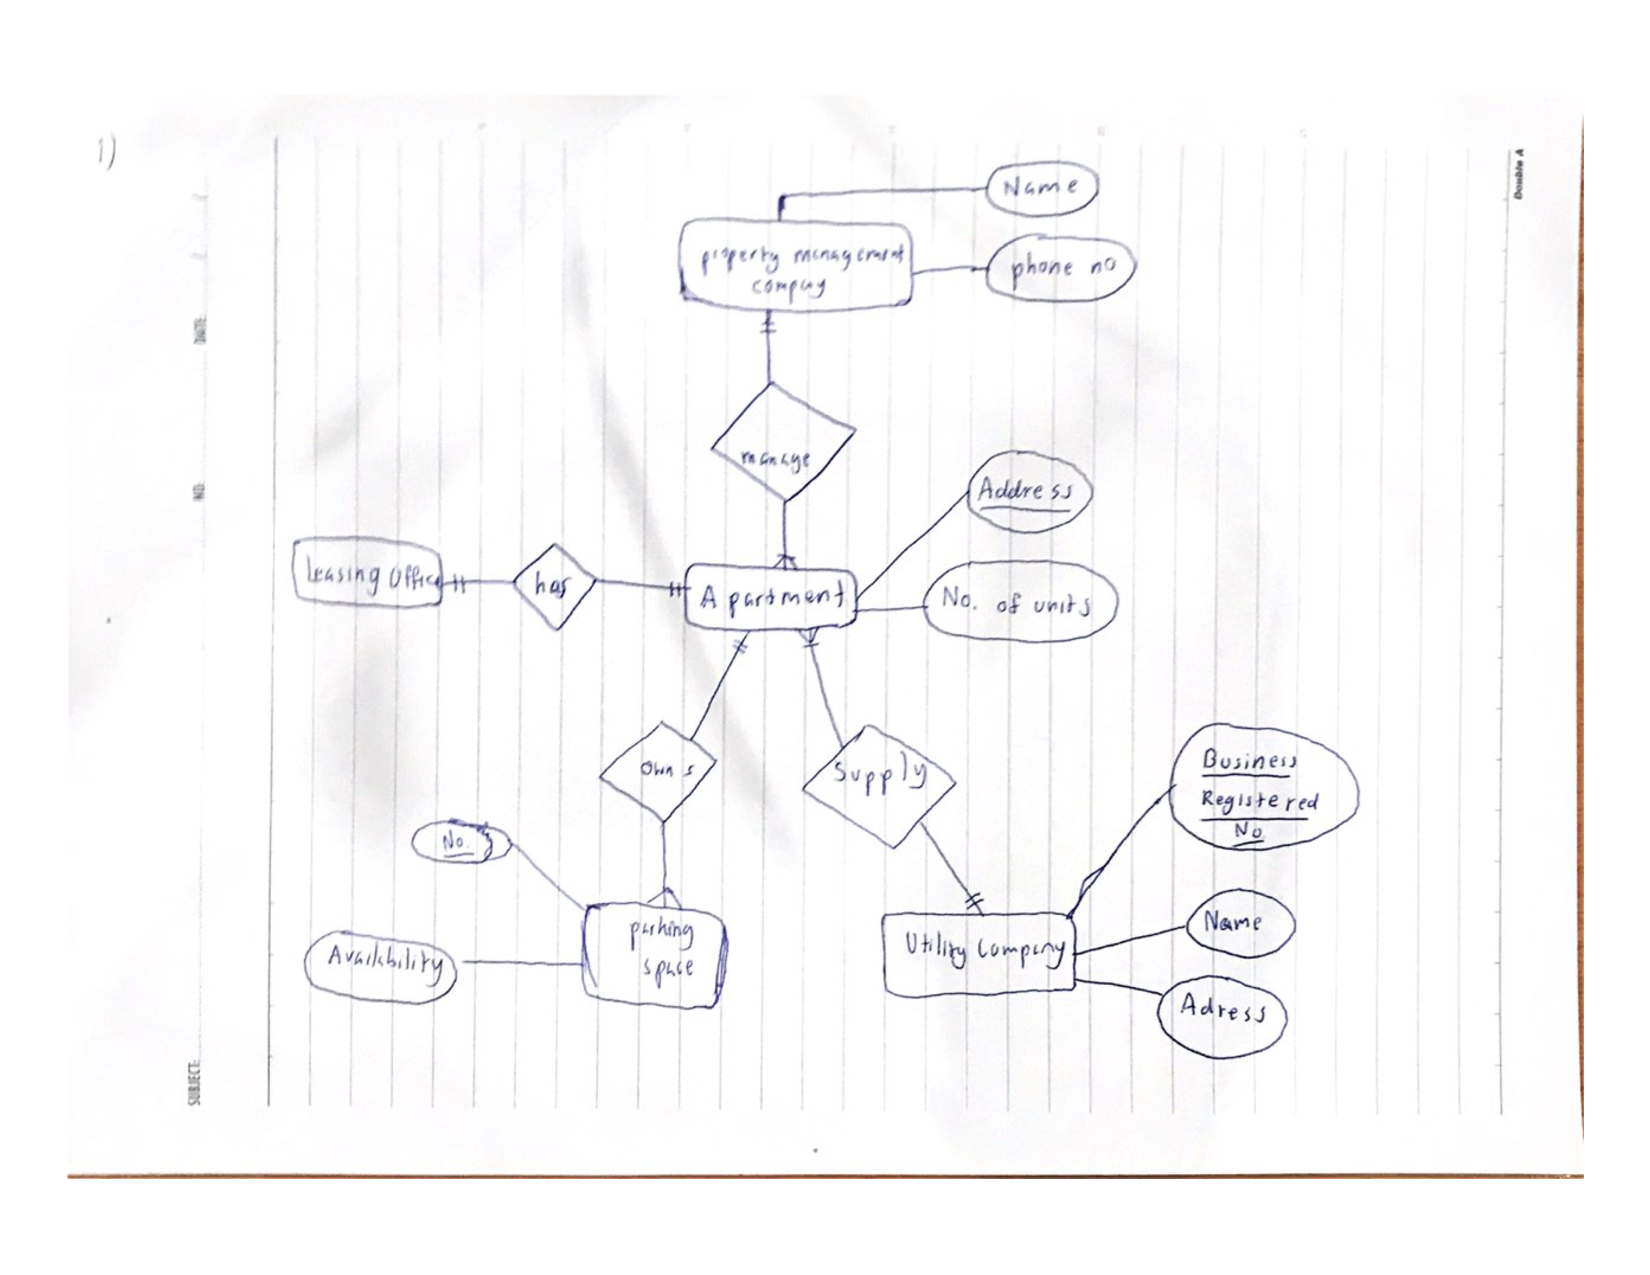
\includegraphics[width=\textwidth]{pic1.pdf}
\part{2}{Relational Database Schema}\\
The relational database schema :\\
PropertyManagementCompany(\underline{Name}: string, Phone:int)\\
Apartment(\underline{Name}: string, No.of unit: int, \underline{Leasing office}:string, Apartment name:string)\\
Parkingspace(\underline{Number}: int ,Availability: string)\\
UtilityCompany(\underline{Business Registered no.}: int ,Name: string ,Address: string)

\question{4}{E/R Diagram}
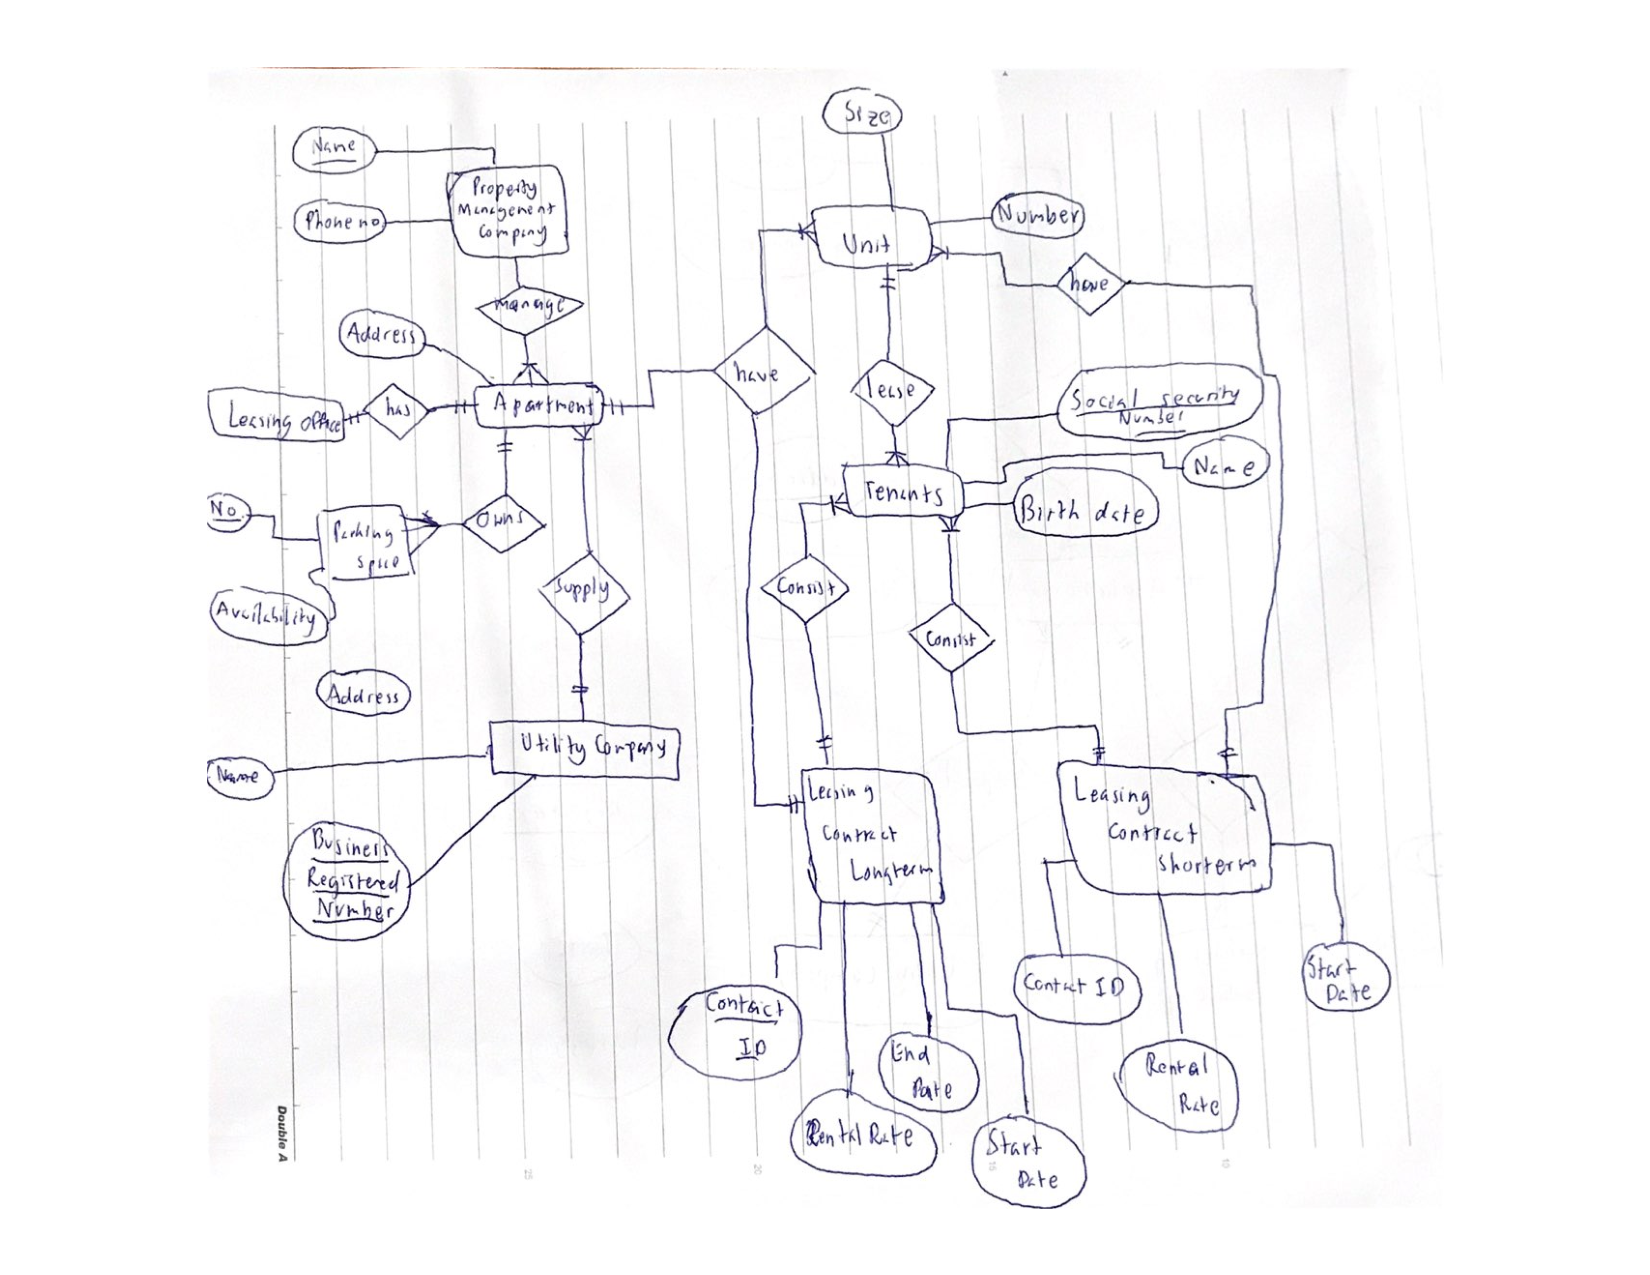
\includegraphics[width=\textwidth]{pic2.pdf}

\question{5}{Relational Model and SQL}
\part{1}{Key and Foreign Key}\\
BEER\\
Primary Key: brand \\
Foreign Key: none \\
COMPANY\\
Primary Key: HQ\_location\\
Foreign Key: Brand\\
BAR\\
Primary Key: name\\
Foreign Key:Brand\_of\_beer\_sold \\
SALE\\
Primary Key: none \\
Foreign Key:Brand\_of\_beer\_sold  and bar

\part{2}{Relational Algebra Expression and SQL}\\
(a) \\ 
SQL:\\
\begin{verbatim}
SELECT brand FROM BEER WHERE country_brewed != country_sold ;
\end{verbatim} 
Relational Algebra:\\
$ \Pi_{brand}(\sigma_{country\_brewed !=country\_sold}(BEER)) $\\
(b)\\
SQL:\\
\begin{verbatim}
SELECT SUM(number_of_sold)  FROM  SALE  GROUP BY year_record ;
\end{verbatim} 
Relational Algebra:\\
$ \Pi_{SUM(number\_of\_sold)}(\sigma\gamma_{year\_record}(SALE)) $\\
(c)\\
SQL:\\
\begin{verbatim}
SELECT brand, name from BAR, BEER where BAR.price_sold > BEER.standard_price ;
\end{verbatim}
Relational Algebra:\\
$ \Pi_{brand,name}(\sigma_{BAR.price\_sold > BEER.standard\_price}(BAR X BEER)) $

\question{6}{SQL}
\part{1}{Find the number of distinct makers for each type of computers}\\
\begin{verbatim}
SELECT DISTINCT maker FROM Computer;
\end{verbatim} 
\part{b}{Find the maker that produced the largest number of computers}\\
\begin{verbatim}
SELECT * FROM 
(SELECT maker FROM Computer ORDER BY (SELECT COUNT(model) 
from Computer GROUP BY maker )) LIMIT 1;
\end{verbatim} 
\part{3}{Without using a sub-query, find a list of PC.model-Laptop.model pairs whose difference in price is less than \$100. Your list should also print the price difference between them}\\
\begin{verbatim}
SELECT compc.model, comlaptop.model,
ABS(comps.price - comlaptop.price) difference FROM computer compc 
INNER JOIN computer comlaptop ON compc.maker=comlaptop.maker
WHERE compc.type='pc' AND comlaptop.type='laptop' AND 
ABS(compc.price - comlaptop.price)<100
\end{verbatim}
\end{document}

